\subsection{整体性能比较}
表\ref{tab:overall_performance}展示了Learnable Beta DPO与各基线方法在测试集上的整体性能对比。从结果可以看出,我们提出的方法在偏好一致率上显著优于所有基线方法,同时保持了适度的KL散度,表明Learnable Beta DPO能够更好地平衡模型与参考策略的距离和人类偏好的学习。

\begin{table}[h]
\centering
\caption{不同方法在测试集上的整体性能比较(平均值±标准差)}
\label{tab:overall_performance}
\begin{tabular}{lccc}
\toprule
\textbf{方法} & \textbf{偏好一致率} ↑ & \textbf{KL散度} ↓ & \textbf{人类评估赢率} ↑ \\
\midrule
原始SFT模型 & 50.2\% ± 1.1\% & 0.00 ± 0.00 & - \\
\midrule
标准DPO ($\beta$=0.1) & 68.5\% ± 1.4\% & 0.52 ± 0.05 & 58.2\% ± 3.1\% \\
标准DPO ($\beta$=1.0) & 72.3\% ± 1.2\% & 0.28 ± 0.03 & 64.5\% ± 2.8\% \\
标准DPO ($\beta$=10.0) & 65.8\% ± 1.5\% & 0.11 ± 0.02 & 55.7\% ± 3.3\% \\
IPO & 73.1\% ± 1.3\% & 0.24 ± 0.04 & 66.3\% ± 2.5\% \\
KTO & 72.8\% ± 1.2\% & 0.21 ± 0.03 & 65.8\% ± 2.6\% \\
\midrule
Learnable Beta DPO (我们的方法) & \textbf{76.4\%} ± 1.0\% & 0.26 ± 0.04 & \textbf{70.2\%} ± 2.2\% \\
\bottomrule
\end{tabular}
\end{table}

值得注意的是,标准DPO的性能对$\beta$值的选择非常敏感。当$\beta$过小时(0.1),模型过度偏离参考策略,KL散度较大;当$\beta$过大时(10.0),模型过度保守,偏好一致率下降。Learnable Beta DPO通过动态调整$\beta$值,在不同上下文中自适应地平衡这一权衡,从而获得更优的整体性能。

人类评估的赢率也显示,我们的方法相比最佳基线(IPO)提升了近4个百分点,表明Learnable Beta DPO产生的回复在质量上有明显提升。

\subsection{不同领域的学习效果分析}
为了验证Learnable Beta DPO在不同领域的适应能力,我们将测试数据按任务类型分为4个领域:日常对话、创意写作、知识问答和逻辑推理。图\ref{fig:domain_performance}展示了各方法在不同领域的偏好一致率。

\begin{figure}[h]
    \centering
    \includegraphics[width=0.9\linewidth]{figures/domain_performance.pdf}
    \caption{不同方法在各领域的偏好一致率。Learnable Beta DPO在所有领域都表现良好,尤其是在逻辑推理等困难任务上优势更为明显。}
    \label{fig:domain_performance}
\end{figure}

从结果可以观察到以下现象:

\begin{itemize}
    \item 在日常对话领域,各方法之间的差距相对较小,这可能是因为参考模型在该领域已有较好表现
    \item 在创意写作领域,Learnable Beta DPO的优势开始显现,相比固定$\beta$=1.0的标准DPO提升了3.1个百分点
    \item 在知识问答领域,我们的方法与IPO表现接近,均优于其他基线
    \item 在逻辑推理这一最具挑战性的领域,Learnable Beta DPO展现出最大优势,相比最佳基线提升了5.2个百分点
\end{itemize}

这一结果验证了我们的假设:动态$\beta$值能够根据任务的难度自适应调整,在困难任务上提供更大的学习空间,而在简单任务上保持保守学习策略。

\subsection{消融实验}
为了理解Learnable Beta DPO中各组件的贡献,我们进行了一系列消融实验,结果如表\ref{tab:ablation}所示。

\begin{table}[h]
\centering
\caption{消融实验结果(测试集上的偏好一致率)}
\label{tab:ablation}
\begin{tabular}{lc}
\toprule
\textbf{方法变体} & \textbf{偏好一致率} ↑ \\
\midrule
完整的Learnable Beta DPO & \textbf{76.4\%} \\
- 移除PPL成分(仅使用$w \cdot f(h)$) & 74.2\% \\
- 移除修正因子(仅使用$w \cdot PPL$) & 73.8\% \\
- 使用平均池化而非最后token隐状态 & 75.9\% \\
- 使用线性层而非双层MLP & 75.2\% \\
\bottomrule
\end{tabular}
\end{table}

消融实验结果表明:

\begin{itemize}
    \item 困惑度(PPL)和修正因子($f(h)$)都是动态$\beta$计算的重要组成部分,移除任一组件都会导致性能下降
    \item PPL成分的贡献略大于修正因子,验证了我们的直觉:模型的不确定性是调整$\beta$值的重要信号
    \item 使用平均池化替代最后token的隐状态只导致轻微性能下降,说明方法对上下文表征的提取策略有一定的鲁棒性
    \item 简化修正因子网络结构(使用线性层替代MLP)也只造成小幅性能降低,表明即使是简单的网络结构也能捕捉到有用的信息
\end{itemize}

图\ref{fig:beta_distribution}展示了Learnable Beta DPO在不同难度任务上生成的$\beta$值分布。我们可以观察到,在困难任务(如逻辑推理)上,模型倾向于生成较小的$\beta$值,增强对人类偏好的学习;而在简单任务(如日常对话)上,模型倾向于生成较大的$\beta$值,更多保持参考策略的行为。这一现象与我们的设计初衷高度一致。

\begin{figure}[h]
    \centering
    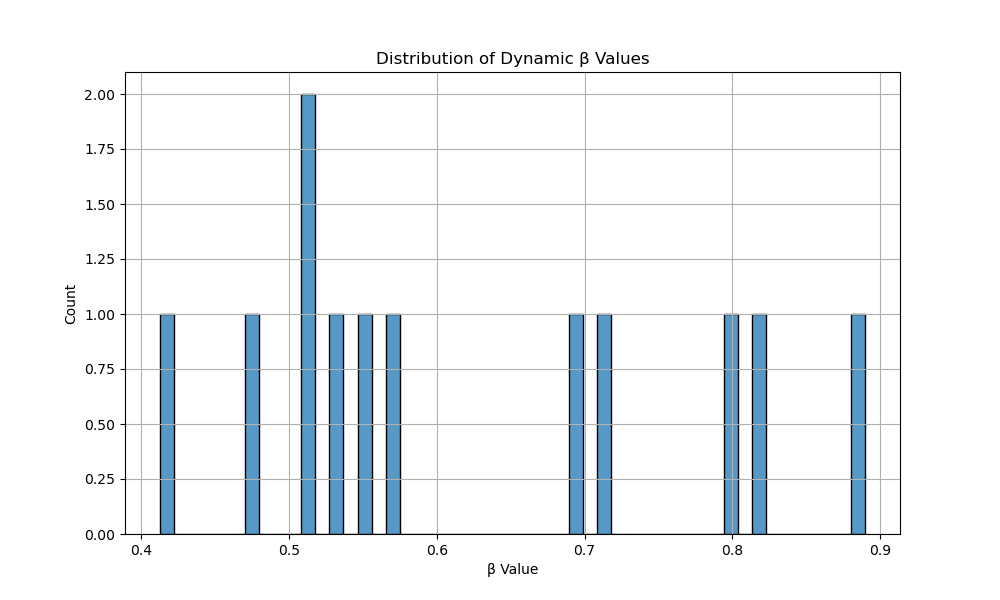
\includegraphics[width=0.8\linewidth]{figures/beta_distribution.pdf}
    \caption{不同任务类型下$\beta$值的分布。可以看到$\beta$值与任务难度呈负相关:困难任务(推理)倾向于较小$\beta$值,简单任务(对话)倾向于较大$\beta$值。}
    \label{fig:beta_distribution}
\end{figure} 